\section{Análisis}
 El presente TFM está enmarcado en un proyecto de investigación,, lo cual implica que no sigue la dinámica clásica de los TFMs de desarrollo de software y productos. En su lugar, en este trabajo se han planteado una serie de problemáticas y posibles soluciones, junto con hipótesis del potencial resultado.

 Por tanto, para demostrar la certeza de dichas hipótesis, se ha desarrollado un conjunto de experimentos que tratan de cumplir una serie de objetivos para establecer patrones/leyes de comportamiento en el en el marco de este trabajo. El único desarrollo de código que se ha llevado a cabo, es el desarrollo de los diferentes scripts que se han encargado de ejecutar las distintas pruebas de cada uno de los experimentos, así como del procesamiento de los datos con los cuales se han generado diversas gráficas.
 
 \subsection{Casos de Uso}
 Debido a la naturaleza investigadora del proyecto, la reutilización de los componentes desarrollados en otros contextos se encuentra condicionada por la dependencia de estos respecto a las características específicas del entorno experimental. Por este motivo, las herramientas con mayor grado de independencia respecto al proyecto son aquellas destinadas a la recopilación y monitorización de métricas de consumo energético. Asimismo, se ha incluido el proceso de cálculo de las características SI y TI sobre un conjunto de vídeos y la posterior generación de una gráfica de dispersión en función de los valores obtenidos, ya que este proceso puede ejecutarse de forma independiente de las características específicas de los experimentos planteados.
 
 A continuación, se presentan los casos de uso identificados junto con sus correspondientes diagramas de actividad, que permiten representar de forma estructurada el funcionamiento de cada uno de estos componentes. 
 
 \subsubsection*{Obtención del Consumo Energético empleando Kepler y Global Energy Meter}
 En la Figura \ref{fig:analisis-kepler-casouso} se observa el caso de uso correspondiente a la recolección de métricas de consumo energético mediante la herramienta \textit{Kepler}, junto con la monitorización realizada en paralelo por \textit{Global Energy Meter}, para un proceso de codificación concreto.
 
 Cada ejecución del script corresponde a un único proceso de codificación asociado a un determinado vídeo. Antes de iniciar la ejecución, es necesario establecer los parámetros correspondientes a la ubicación de los archivos en los que se almacenarán las métricas, el nombre o identificador del experimento y el tipo de configuración de codificación empleada, indicando si la carga se ejecutará exclusivamente sobre la CPU o mediante una configuración combinada de CPU y GPU.
 
 \begin{figure}[H]
 \centering
 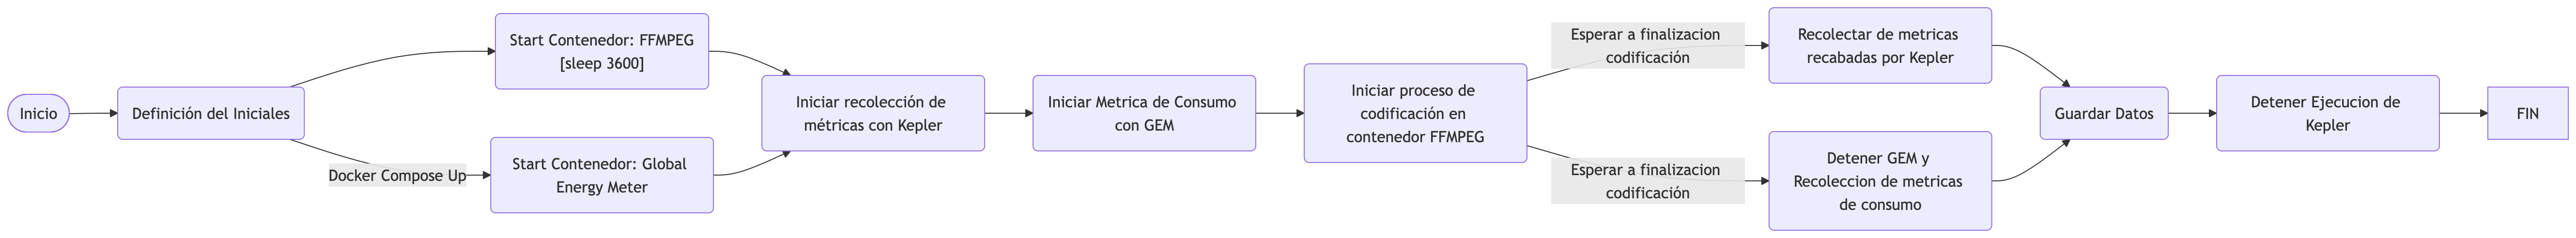
\includegraphics[width=\linewidth]{figs/kepler-caso-uso.png}
 \caption{Diagram de funcionamiento interno del script encargado de la recolección de métricas con Kepler y Global Energy Meter}
 \label{fig:analisis-kepler-casouso}
 \end{figure}
 
 \subsubsection*{Obtención del Consumo Energético empleando Scaphandre y Global Energy Meter}
 Para este caso de uso se emplea la herramienta \textit{Scaphandre} para llevar a cabo la recopilación de métricas de consumo energético, representado en la Figura \ref{fig:analisis-scp-casouso}. Al igual que en el caso de uso anterior, \textit{Global Energy Meter} realiza de forma paralela la recopilación de métricas a nivel de nodo, que posteriormente se utilizarán como referencia para comparar los resultados obtenidos mediante \textit{Scaphandre}.
 
 El funcionamiento de este script se basa en el desarrollado para \textit{Kepler}, por lo que ambos presentan una estructura de ejecución prácticamente idéntica. El script se ejecuta una vez por cada proceso de codificación cuyo consumo se desee monitorizar. Antes de iniciar cada ejecución, es necesario definir los parámetros correspondientes al tipo de codificación realizada, así como el directorio de destino en el que se almacenarán las métricas recopiladas. De este modo, cada ejecución genera un conjunto de datos asociado a una configuración concreta de codificación, facilitando posteriormente su identificación y análisis.
 
 \begin{figure}[H]
 \centering
 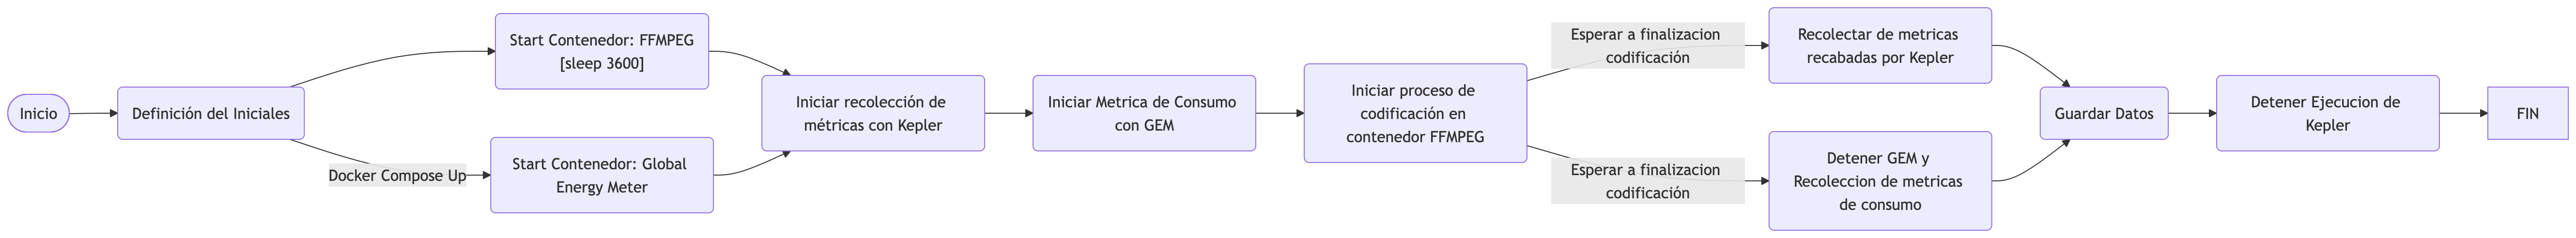
\includegraphics[width=\linewidth]{figs/kepler-caso-uso.png}
 \caption{Diagram de funcionamiento interno del experimento 1.2 recolección de métricas con Scaphandre y Global Energy Meter}
 \label{fig:analisis-scp-casouso}
 \end{figure}
 
 \subsubsection*{Obtención de Consumo Energético con Container Energy Monitoring y Global Energy Meter}
 Para el caso de uso correspondiente a la toma de métricas de consumo mediante la herramienta \textit{Container Energy Monitoring}, se ha modificado el proceso de ejecución para permitir la realización de múltiples iteraciones de forma automatizada. Antes de iniciar la ejecución, se debe definir el número de iteraciones que se realizarán y un identificador que permita distinguir el conjunto de mediciones obtenidas. Asimismo, se establece la estructura de directorios en la que se almacenarán los datos generados durante las pruebas.
 
 De este modo, el script ejecuta el proceso de monitorización y almacenamiento de las métricas un total de $n$ veces, donde $n$ corresponde al número de iteraciones definido previamente a la ejecución. Esto permite automatizar la repetición de las mediciones y mantener organizados los datos correspondientes a cada conjunto de pruebas. A continuación, se muestra en la Figura \ref{fig:cem-scp-casouso} el diagram de ejecución del caso de uso descrito.
 
 \begin{figure}[H]
 \centering
 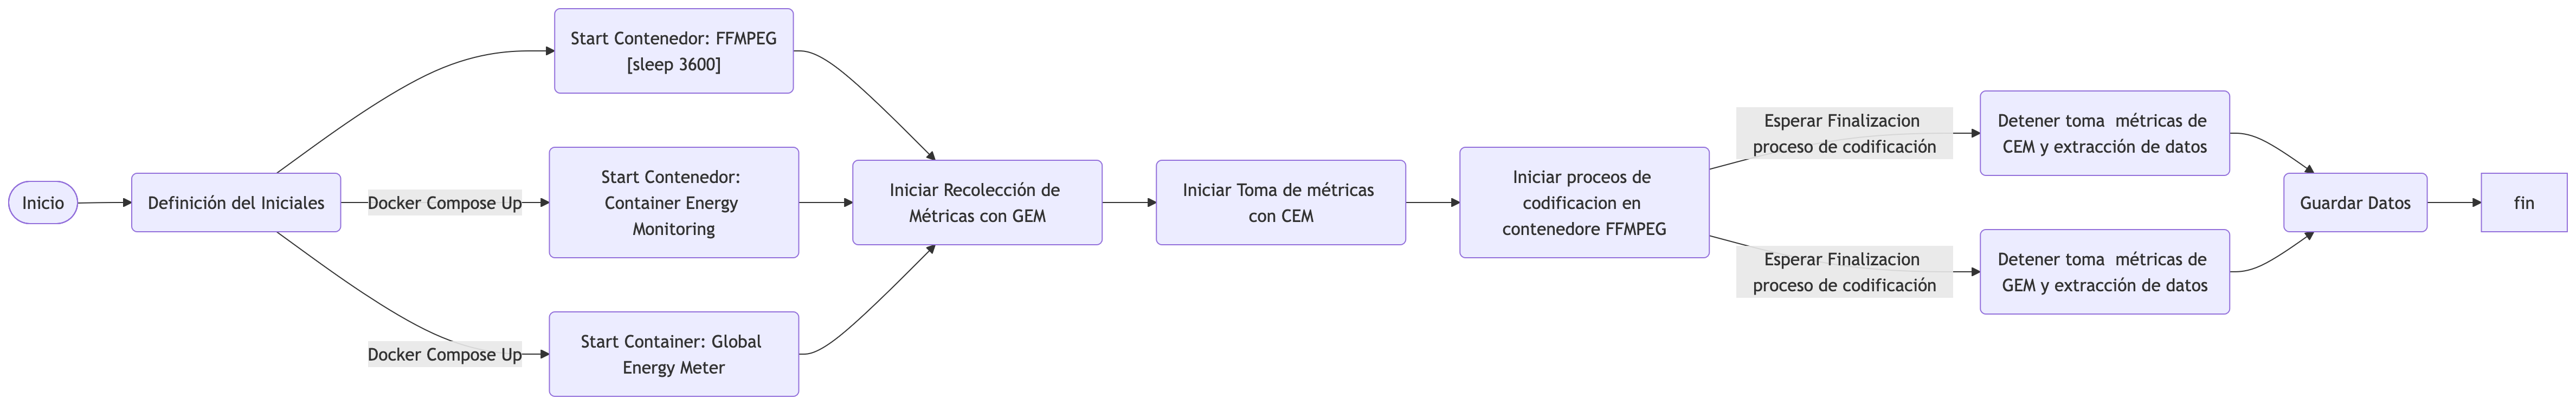
\includegraphics[width=\linewidth]{figs/cem-caso-uso.png}
 \caption{Diagram de funcionamiento interno del experimento 1.2 recolección de métricas con Container Eneregy Monitoring y Global Energy Meter}
 \label{fig:cem-scp-casouso}
 \end{figure}
 
 
 \subsubsection*{Seleccionar segmentos de 10 segundos que tengan un SITI similar}
 En el siguiente caso de uso se muestra el diagrama básico del script encargado de calcular las características SI y TI de los chunks de video, siendo la Figura \ref{fig:siti-chunks-casouso} el correspondiente diagrama de ejecución. Una vez obtenidos estos valores, se empleará otro script para generar una gráfica de dispersión que represente la distribución de los chunks en función de sus características espaciales y temporales. Sobre esta representación se definirán las diferentes zonas de interés y se realizará la selección de los chunks que posteriormente se utilizarán para construir los vídeos con las características requeridas en cada uno de los experimentos.
 
 \begin{figure}[H]
 \centering
 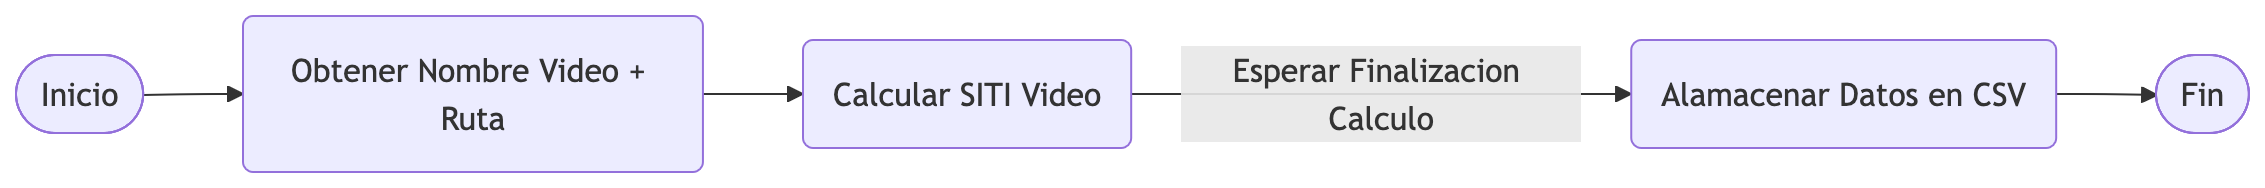
\includegraphics[width=\linewidth]{figs/sitichuncks.png}
 \caption{Diagrama de ejecución el SITI de los fragmentos de videos disponibles para experimentar}
 \label{fig:siti-chunks-casouso}
 \end{figure}
 
\section{Diseño del proyecto}
El flujo de ejecución de los experimentos se mantiene uniforme a lo largo del estudio. En primer lugar, se ejecutan las pruebas mediante scripts de automatización en Bash; posteriormente, los datos recopilados se procesan en Python para generar la gráfica y métricas correspondientes. Finalmente, se realiza un análisis cuantitativo de los resultados y se redactan las conclusiones parciales que estructuran la síntesis final del trabajo.

En cada experimento se iterará sobre un conjunto de variables independientes, cuyos valores específicos se ajustan según el contexto de la prueba:

\begin{itemize}
    \item \texttt{Herramienta de toma de métricas:} Variable exclusiva del \textit{Experimento 1 (Selección de Herramienta)}. Se evalúan las soluciones \textit{Kepler}, \textit{Scaphandre} y \textit{Container Energy Monitor} para determinar cuál ofrece mayor precisión al monitorizar procesos en contenedores.

    \item \texttt{Tasa de bits (Bitrate):} Variable clave en los Experimentos 2 y 3. Rango de valores en Mbps según el estándar del códec (H.264 o H.265), detallado en la Tabla \ref{tab:ana-bitrate-values}.

    \item \texttt{Codificadores y base hardware:} Configuración evaluada en los Experimentos 2 y 3, abarcando ejecuciones sobre CPU pura y aceleración por GPU física (Tabla \ref{tab:exp2-codecs-selection}).

    \item \texttt{Complejidad espacial y temporal (SI y TI):} Métricas empleadas en el Experimento 2 para analizar la correlación entre la carga del video y el consumo energético. Los videos del dataset se clasifican en cuatro cuadrantes de complejidad: \textit{HTI\_HSI}, \textit{HTI\_LSI}, \textit{LTI\_HSI} y \textit{LTI\_LSI}.

    \item \texttt{Asignación de recursos (Cores y Threads):} Límite de núcleos de CPU asignados al contenedor y número de hilos de ejecución en el codificador, evaluado en el Experimento 3 para determinar el punto de saturación y eficiencia energética.
\end{itemize}

\begin{table}[H]
\centering
\begin{minipage}{0.48\textwidth}
  \centering
  \begin{tabularx}{\linewidth}{|>{\centering\arraybackslash}X|>{\centering\arraybackslash}X|>{\centering\arraybackslash}X|}
    \hline
    \rowcolor[HTML]{C0C0C0} 
    \textbf{Codificador} & \textbf{Experimento 2 (Mbps)} & \textbf{Experimento 3 (Mbps)} \\ \hline
    \cellcolor[HTML]{EFEFEF}libx264 / h264\_nvenc & 10, 20, 25, 30, 35, 40, 50 & 10, 30 \\ \hline
    \cellcolor[HTML]{EFEFEF}libx265 / hevc\_nvenc & 10, 15, 20, 25, 30, 35, 40 & 10, 30 \\ \hline
  \end{tabularx}
  \caption{Rango de bitrate (Mbps) seleccionado para cada estándar con el cual se llevarán a cabo los experimentos de codificación de vídeo y consumo energético.}
  \label{tab:ana-bitrate-values}
\end{minipage}%
\hfill
\begin{minipage}{0.48\textwidth}
  \centering
  \begin{tabularx}{\linewidth}{|>{\columncolor[HTML]{EFEFEF}\centering\arraybackslash}X|>{\centering\arraybackslash}X|>{\centering\arraybackslash}X|}
    \hline
    \rowcolor[HTML]{C0C0C0}
    \textbf{Códec} & \textbf{CPU Host} & \textbf{GPU} \\ \hline
    libx264     & X & - \\ \hline
    libx265     & X & - \\ \hline
    h264\_nvenc & X & X \\ \hline
    hevc\_nvenc & X & X \\ \hline
  \end{tabularx}
  \caption{Selección de los codificadores de los estándares H.264 y H.265, con los que se llevará a cabo los experimentos de codificación de vídeo y recolección de métricas de consumo}
  \label{tab:exp2-codecs-selection}
\end{minipage}
\end{table}
 
\subsection{Validación de Resultados}

% VALIDACION DE LOS RESULTADOS
En esta seccion se incluyen el conjunto de equaciones utlizadas para determinar diversas cuestiones comparativas, como el porcentaje de mejora entre herramientas o diferencias percentuales entre métricas.

La primera de las ecuaciones determina la desviación porcentual en la estimación de consumo de energía del nodo de una herramienta frente al valor que se obtiene con Global Energy Meter (GEM) \ref{eq:percent-energy-node}:

\[E\%_{porcentaje\_energia\_GEM} = \frac{E_{GEM}-E_{Herramienta}}{E_{GEM}}*100 \label{eq:percent-energy-node}\]

La segunda de las ecuaciones determina la desviación porcentual en la estimación de consumo de energía del proceso (o procesos en el caso de que haya concurrencia) que ofrece una herramienta frente al valor que se obtiene con Global Energy Meter (GEM) \ref{eq:percent-energy-tool_node}:

\[E_{\textrm{energía\_proceso}} = 100 * \frac{E_{\textrm{GEM}} - E_{\textrm{proceso\_herramienta}}}{E_{\textrm{GEM}}} \label{eq:percent-energy-tool_node}\]

\section{Configuración de Entorno \& Herramientas}\label{exp0-environment}
% Seleccon de S0 
\subsection{Seleccion e Intalacion del Sistema Operativo}
%DONE
En un principio se decidió instalar el sistema operativo XUbuntu 26.04 en base a la recomendación de mi tutor de TFM, Juan Gutiérrez Aguado, ya que es un sistema operativo que él utiliza diariamente y sobre el que tiene una vasta experiencia de uso. Esto proporciona una capa extra de seguridad y de conocimiento sobre el entorno en el que se desarrollarían las pruebas, además del resto de recursos de conocimiento oficiales y no oficiales que existen sobre este sistema operativo.

Una vez finalizada la instalación, se hizo uso del gestor de versiones de drivers interno de Ubuntu, llamado 'ubuntu-drivers', para instalar la versión de los drivers de NVIDIA más compatible con la tarjeta gráfica NVIDIA Quadro M4000. Al comprobar si se podía acceder a los datos internos de consumo mediante nvidia-smi, se obtuvo un error que indicaba que no era capaz de comunicarse con la API interna de la tarjeta gráfica. Al revisar los mensajes proporcionados por el kernel, se pudo determinar que se trataba de un problema de compatibilidad de los drivers con la versión del kernel. Por este motivo se decidió instalar la versión 24.04 de XUbuntu, la cual hace uso de la versión 6.14 del kernel, solventando el problema de compatibilidad de los drivers.

Una vez reinstalado el sistema operativo, se procedió a reinstalar nuevamente los drivers de NVIDIA junto con los paquetes requeridos por nvidia-smi, de la misma forma que con la versión anterior. De nuevo, al tratar de acceder a los datos de consumo mediante `nvidia-smi`, apareció el mismo problema, pero al revisar los mensajes del kernel, se indicaba que el error no era de compatibilidad, sino la ausencia de un componente concreto llamado 'nvidia-drm'. Este componente forma parte del conjunto de módulos del kernel de NVIDIA que permite al kernel comunicarse con la tarjeta gráfica de NVIDIA \cite{nvidia-drm-documentation}. Al tratar varias veces de reconstruir el módulo manualmente, sin lograr éxito, se optó por buscar información en foros oficiales de NVIDIA y foros de la comunidad Ubuntu y Xubuntu, llegando a la conclusión de que era un problema que sucedía en algunas versiones de XUbuntu debido a dos razones principales: La versión Nouveau de los drivers ,y la incompleta compatibilidad de los drivers con XUbuntu.\

El primer problema estaba relacionado con el controlador libre Nouveau, desarrollado por la comunidad mediante técnicas de ingeniería inversa. Aunque este controlador proporciona compatibilidad básica con un amplio número de tarjetas gráficas NVIDIA, no implementa completamente las funcionalidades propietarias ofrecidas por los controladores oficiales, entre ellas la interfaz NVML, utilizada por herramientas como nvidia-smi para acceder a métricas avanzadas de la GPU, incluido el consumo energético. Para solucionar este problema fue necesario deshabilitar la carga del módulo Nouveau y reinstalar exclusivamente los controladores oficiales proporcionados por NVIDIA.\

El segundo problema estaba relacionado con el mecanismo de instalación automática de controladores proporcionado por la utilidad ubuntu-drivers. Tras consultar la documentación oficial y diferentes foros de las comunidades de Ubuntu y Xubuntu, se comprobó que esta herramienta puede instalar automáticamente la versión más reciente del controlador junto con paquetes pertenecientes a versiones diferentes o dejar dependencias de instalaciones anteriores. Esta situación puede provocar inconsistencias entre los módulos del kernel y las bibliotecas de usuario, impidiendo que componentes como nvidia-drm o nvidia-smi funcionen correctamente. Como consecuencia, fue necesario eliminar completamente todos los paquetes relacionados con NVIDIA y realizar una instalación manual de una versión del controlador compatible con la tarjeta gráfica y con el sistema operativo empleado.\

Pese a todo ello, no se logró una comunicación adecuada con la API interna de la tarjeta gráfica, lo que impidió el acceso a las métricas de consumo energético mediante nvidia-smi. Es por ello que se optó por instalar otra distribución de Linux más flexible, con mayor compatibilidad con los drivers de NVIDIA. Finalmente, se decidió instalar Debian, ya que cumplía con los requerimientos necesarios, además de ser una distribución que a lo largo de los años personalmente había utilizado para diferentes proyectos; por tanto, tenía experiencia de uso y conocía su funcionamiento interno y su filosofía de trabajo.\

%PENDIENTE
La versión de Debian seleccionada una version 2 releases por detras de la version actual (Duke - 15)\cite{debian-releases}, siendo la version 13(Trixie) la seleccionada para la instalacion. Durante la instalacion, se decidio marcar la autodeteccion de tarjeta grafica y la instalacion automatica de drivers de NVIDIA.


% Instalacio de requerimeintos del sistema para pruebas
%   - Nvidia Drivers  
%   - Nvidia SMI
%   - Nvidia Container Toolkit
%   - Docker 
% Seleccion de Herramientas de metricas 
%  - Criterio de Sleccion
%  - Repos Visitados
%  - Papers consultados
% Instalacion y Uso de herramientas
%   - Container de linux-server ffmpeg 
%   - Container de Juan EM
%   - Kepler
%         - Problemas y Modificacion de kepler manual - libnvida-ml
%   - Scaphandre Container

 


